\section{One Dimension}

This section covers the computing of functions of a single random variable. The following serve as motivating examples,
\begin{enumerate}
\item $X^2$
\item $log(X)$
\item $\frac{1}{X}$
\item $\frac{1}{log(X^2-X)}$
\item $[X-k]^+ - [X-k]^- \equiv X - k$
\label{example:motivating_examples}
\end{enumerate}

An interesting feature of the last item, known as Put-Call Parity \cite{dineen00}, is that it seems to recover lost information through truncation. If $Z_+ := [X-k]^+$ and $Z_- := [X-k]^-$ then $Z_+$ and $Z_-$ are maximally correlated. In the language of quantum mechanics the two $Z$'s are \emph{maximally entangled}. \todo{find reference}

As a naming convenience it is assumed that $X$ represents a \emph{basic random variable}. A basic random variable is on that is not related to any other random variable within RICO by an explicit function. Conversely the label $Z$ refers to a random variable that is functionally related to some $X$ via an explicit function $f$ such that $Z = f(X)$. When more than one function of $X$ is needed they will be distinguished by subscripting. Since a random variable is defined by its associated cumulative density function RICO requires random variables to be associated with the following computable expressions
\begin{align}
P(Z < k) && P(Z = k)
\label{exp:required_expressions}
\end{align}
for any constant $k$. In order to incorporate functions of random variables into an algorithmic context is it also necessary to be able to compute
\begin{align*}
P(Z_1 < Z_2) && \text{ where } && Z_1 = f_1(X),\: Z_2 = f_2(X)
\end{align*}
Notice that $P(Z_1 < Z_2) = P(Z_1 - Z_2 < 0)$ and that $Z_1 - Z_2$ is itself a random variable. The computable expressions in (\ref{exp:required_expressions}) are sufficient to compute $P(Z_1 < Z_2)$ which may arise in conditional branching statements such as $if(Z_1 < Z_2) \{...\}$. Both branches of an \emph{if} statement may be followed albeit with different associated probabilities. Conditional branching statements will be discussed in a later section.

\subsection{Plotting $Z = f(X)$}

A \emph{continuous} random variable has the property that
\begin{align}
P(X = k) = 0 \;\forall \;k \in \mathcal{D}(X)
\label{prop:conditional_random_variable}
\end{align}
and it assumed by RICO that a continuous random variable has an associated probability density function, $\rho(X)$. The expression $\mathcal{D}(X)$ refers to the support of $X$ which in the continuous case is the domain of the associated probability density function.

A \emph{discrete} random variable has discrete support such that
\begin{align}
P(X = k_i) = p_i \;\forall\;k_i \in K = \{k_1, k_2, \dots, k_n\}
\label{prop:discrete_random_variable}
\end{align}

In general a random variable $X$ may be a mixture of continuous and discretely ditributed probability. In RICO the continuous and discrete aspects of a random variable are represented separately. The continuous aspect of a random variable is more numerically challenging and will be the focus of this section as a special case. 

Notice that the discrete aspect of a random variable cannot be ignored even if an original $X$ is purely continuous. Consider the motivating example, $Z = [X-k]^+$ in (\ref{example:motivating_examples}), transforms a continuous $X$ into a \emph{mixed} continuous/discrete $Z$.

In the next section it is assumed that both $X$ and $Z = f(X)$ are continuous random variables.

\subsubsection{Plotting Continuous $Z = f(X)$}

To plot the probability density function of $Z = f(X)$ it is assumed that a software module will be employed to render the actual graph for the user and that the module requires an array of pairs of points, 
\begin{align}
\{(z_i, h_i)\}_{i=1}^n
\label{exp:graph_list}
\end{align}
where $z_i$ is a point in the support of $Z$ and $h_i = \rho(z_i)$, the probability density of $Z$ at $z_i$. The associated probability density function of $Z$ is denoted $\rho(Z)$. 

To first approximation the values of each $h_i$ are found by choosing a set of partition endpoints 
\begin{align*}
(z_i^p)_{i=1}^n \subset \mathcal{D}(Z)
\end{align*}
so that 
\begin{align*}
z_i \in (z_i^p, z_{i+1}^p)
\end{align*}
and the $h_i$ are approximated as
\begin{align*}
h_i = \frac{p_i}{z_{i+1}^p - z_i^p} && \text{ where } p_i = P(z_i^p < Z < z_{i+1}^p) && i = 1,\dots,n
\end{align*}
A \emph{partition of $Z$} is understood to be a partition of the range of $f(X)$.

\begin{figure}
  \centering
  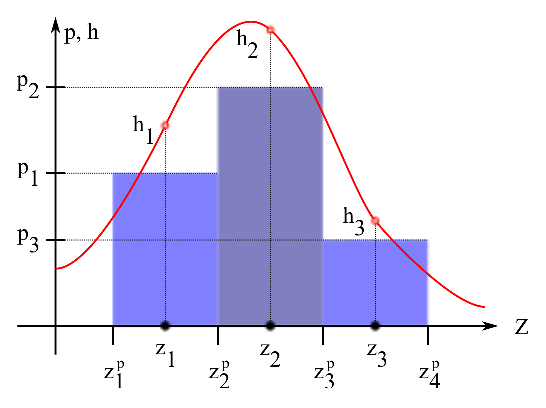
\includegraphics{Images/Zpartition4.eps}
  \caption[Three point Partition of $Z$]
          {Three point Partition of $Z$}
  \label{fig:Zpartition4}
\end{figure}

The relationship between the partition elements is shown in figure \ref{fig:Zpartition4}. Assuming $n \ge 2$ the $z_i^p$ partition points are computed in RICO as midpoints of the $(z_i)_{i=1}^n$ array
\begin{align*}
z_i^p = \begin{cases}
       z_1 - \frac{1}{2}(z_1 + z_2) & \text{ if } i = 1\\
       \frac{1}{2}(z_{i-1} + z_i) & \text{ if } 1 < i \le n\\
       z_n + \frac{1}{2}(z_{n-1} + z_n) & \text{ if } i = n+1\\
      \end{cases}
\end{align*}
Let the associated partition of $Z$ be
\begin{align*}
Z^p =(-\infty, z_1^p, z_2^p, ..., z_{n+1}^p, \infty)
\end{align*}

Since $Z$ is a purely continuous random variable the \emph{partition elements} of $Z^p$ are assumed in RICO to be open intervals. The missing endpoints of the partition elements form a set of probability zero. Let the partition elements of $Z^p$ and associated probability values be indexed as
\begin{align*}
Z_0^p &= (-\infty, z_1^p) && p_0 = P(Z_0^p)\\
Z_i^p &= (z_i^p, z_{i+1}^p) && p_i = P(Z_i^p) && i = 1, \dots, n\\
Z_{n+1}^p &= (z_{n+1}^p, \infty) && p_{n+1} = P(Z_{n+1}^p)
\end{align*}

\subsubsection{Numerical Considerations}

\begin{figure}
  \centering
  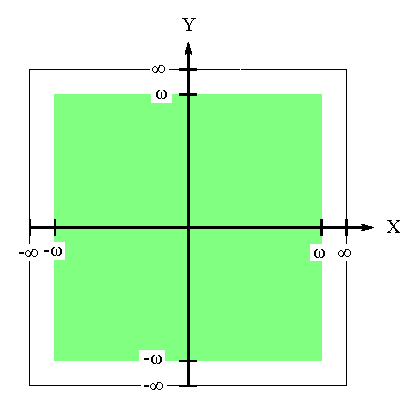
\includegraphics{Images/Quadrants.eps}
  \caption[Fundamental Numeric Domain]
          {Fundamental Numeric Domain}
  \label{fig:Quadrants}
\end{figure}

Numerically, real numbers are represented by a finite number of floating point values. Let $\Omega$ be the largest representable floating point value. Similarly let $\iota$ be the smallest positive floating point value. In RICO, a constant called $\omega$ is defined as
\begin{align}
\omega = min \left\{\Omega, \frac{1}{\iota} \right\}
\label{constant:omega}
\end{align}
and let $\epsilon$ be the smallest numerically representable positive probability value. One purpose for defining $\epsilon$ is so that so-called \emph{thin tailed} probability distribution such as the Gaussian may be represented using a finite support interval as in
\begin{align*}
\mathcal{D}(X) = (X_{min}, X_{max})
\end{align*}
where $-X_{min} = X_{max} \approx 10$, depending on $\epsilon$. The $X_{min}$ and $X_{max}$ satisfy the following relations
\begin{align*}
P(X < X_{min}) \le \epsilon && P(X_{max} < X) \le \epsilon
\end{align*}

In particular all functions of a random variable have domain and range in $(-\omega, \omega)^2$ as represented visually by the shaded region in figure \ref{fig:Quadrants}.

\subsubsection{Functions of Random Variables}

In RICO there are several types of functions; \emph{primitive}, \emph{composite} and \emph{piecewise monotonic}. Both primitive and composite functions are described elsewhere. An relevant feature of a primitive function such as $x^2, log(x)$, etc. is that it has a \emph{primitive domain}. A primitive domain is a traditional mathematic domain. For example the primitive domain of $x^2$ is the interval $(-\infty, \infty)$ and for $log(x)$ the primitive domain is $(0,\infty)$. And example of a composite function is $x^2-x$, a function composed of other composite functions, primitive functions and RICO-supported operations such as addition, subtraction, multiplication, etc.

In RICO, a piecewise monotonic function $f(X)$ of a random variable $X$ is set of \emph{piecewise monotonic function elements}. A piecewise monotonic function element is a domain interval and either another piecewise monotonic function element, a composite function or a primitive function. The set of piecewise monotonic function domain intervals form a non-intersecting set denoted $\mathcal{D}(Z)$ where $Z = f(X)$. The implied partition of the domain space is a set of open intervals containins $\mathcal{D}(Z)$ and denoted $Z^p$. The $Z^p$ set is described above in the context plotting $f(X)$ and is defined here via
\begin{align*}
\mathcal{D}(Z)_j = z_i^p \in Z^p && \text { for some } i \in 1, \cdots, n \text{ and } j \in 1, \cdots, m
\end{align*}
For example, if $f(X) = [X-k]^+$ then
\begin{alignat*}{2}
\mathcal{D}(Z)_1 &= (-\infty, k), &\quad \mathcal{D}(Z)_2 &= (k, \infty)\\
f_1(x) &= 0,  &f_2(x) &= x
\end{alignat*}
where $f_1$ and $f_2$ are primitive functions.

Notice that the recursive nature of the definition of a piecewise monotonic function forms a tree structure denoted $\mathcal{T}(f)$. The leaf nodes of $\mathcal{T}(f)$ are piecewise monotonic elements whose associated functions are either composite of primitive. A critical aspect of the definition of a piecewise monotonic function in RICO is that leaf node functions are monotonic over their associated domain interval. For example the primitive function $f(x) = x^2$ has the associated primitive domain $(-\infty, \infty)$, but the piecewise monotonic function $f(x) = x^2$ is composed of two elements,
\begin{align}
f(x) = \begin{cases}x^2 \text{ if } x \in (-\sqrt{\omega}, 0)\\
                    x^2 \text{ if } x \in (0, \sqrt{\omega})
       \end{cases}
\label{equation:x2}
\end{align}
where the numerical considerations described in the previous section are taken into account.

\subsubsection{Piecewise Monotonic Functions of Random Variables}

\begin{figure}
  \centering
  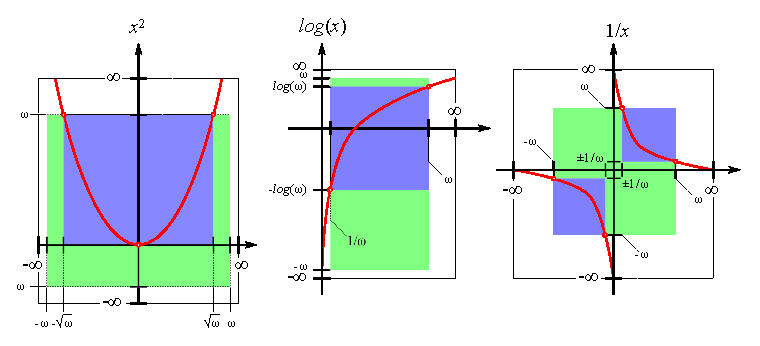
\includegraphics{Images/ExampleDomains.eps}
  \caption[Refined Domains of Primitive Functions]
          {Refined Domains of Primitive Functions}
  \label{fig:ExampleDomains}
\end{figure}

For the purpose of plotting an other analysis such as computing $P(Z < k)$ for $Z = f(X)$ a composite $f$ must be transformed into a piecewise monotonic $f$. The transformation process is referred to as \emph{refinment}. Function refinment serves two purposes. The first is to ensure that the numerical considerations are respected such that the associated function evaluates to a representable floating point value for every element of the domain. The second purpose is to ensure monotonicity within each domain interval.

\begin{figure}
  \centering
  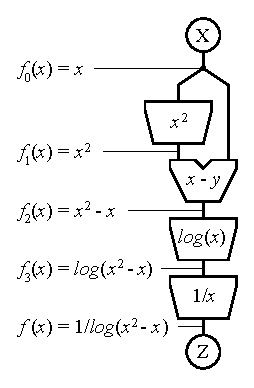
\includegraphics{Images/invlogX2minusXflow.eps}
  \caption[Parse Tree of $Z = 1/log(X^2 - X)$]
          {Parse Tree of $Z = 1/log(X^2 - X)$}
  \label{fig:invlogX2minusXflow}
\end{figure}

The refinment for several primitive functions is depicted in figure \ref{fig:ExampleDomains}  As a guiding example of the refinment process suppose that
\begin{align*}
Z = f(X) = \frac{1}{log(X^2 - X)}
\end{align*}
where
\begin{align*}
X \sim Normal(0,1) \text{ and } \mathcal{D}(X) = (-10,10)
\end{align*}
The parse tree of $f$ is a composition of primitive functions, composite function and arithmetic operator components is shown in figure \ref{fig:invlogX2minusXflow}. Transforming the composite $f$ into the piecewise monotonic $f$ is a sequention process that begins at the input $X$. Several composite function components are identified in figure \ref{fig:invlogX2minusXflow} including the indentity function $f_0(x) = x$. 

\begin{figure}
  \centering
  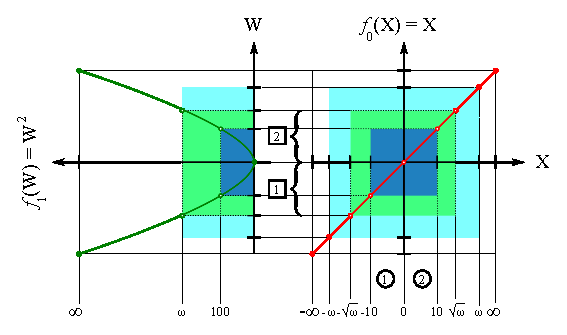
\includegraphics{Images/X.eps}
  \caption[Refinement $f_0(X)$ by $f_1(X)$]
          {Refinement $f_0(X)$ by $f_1(X)$}
  \label{fig:X}
\end{figure}

To begin, note that the domain of $X$ is the interval $(-10,10)$ which is assigned to be the domain of $f_0$. The next step is to consider the effect of $f_0$ of the adjacent node $x^2$ and the $y$-input of the operation $x-y$. Assume that $f_1(x)$ is refined in isolation of the containing $f(x)$ so that its initial definition is given in equation \ref{equation:x2}. The refinment process is to take the range of $f_0$, $(-10,10)$, and intersect it with the domain of $f_1$ into range components $\{(-10,0), (0,10)\}$ and find the pre-image under $f_0$ which is also $\{(-10,0), (0,10)\}$. This process is shown in figure \ref{fig:X} where \squared{1} = $(-\sqrt{\omega}, 0)$, \squared{2} = $(0, \sqrt{\omega})$, \circled{1} = $(-10,0)$, \circled{2} = $(0,10)$. 

In isolation the operation $x-y$ accepts any input in $(-\omega, \omega)$ so no further refinement is needed at this stage. Similarly no further refinement of $f_2$ is imposed by $x-y$. The domain of $f_2$ is then the set \{\circled{1}, \circled{2}\} in figure \ref{fig:X}.


\begin{figure}
  \centering
  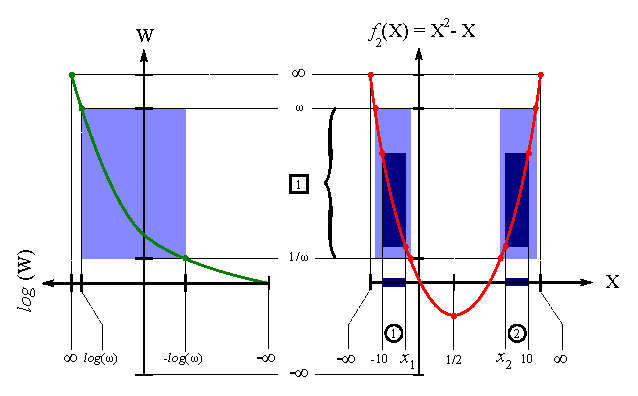
\includegraphics{Images/X2minusX.eps}
  \caption[Domain of $f_2(X)$]
          {Domain of $f_2(X)$}
  \label{fig:X2minusX}
\end{figure}

The domain of $f_2$ in the parse tree \ref{fig:invlogX2minusXflow} is refined by the domain of the primitive $log(x)$. Because $f_2$ involves a $2\times1$-dimensional transform, namely subtraction, and since the two operands are maximally entangled, the domain is less clearly defined and must be identified numerically. In general any value can be achieved by the transform $x-y$. Referring to the figure \ref{fig:X2minusX} the domain of $log(x)$ is \squared{1} = $(1/\omega, \omega)$. The domain of $f_2(X)$ is notated as before,
\begin{align*}
\mathcal{D}(f_2) &= \mathcal{D}(f_1) \cap f_2^{-1}(\mathcal{D}(log))\\
                    &= (-10,10) \cap \left((-\sqrt{\omega}, x_1) 
                                            \cup (x_4, \sqrt{\omega})\right)\\
                    &= (-10, x_1)  \cup (x_2, 10)
\end{align*}
where
\begin{align*}
x_1 = min \left\{ -f_2^{-1}(1/\omega),  -\frac{1}{\omega} \right\} && 
x_2 = max \left\{ +f_2^{-1}(1/\omega), 1+\frac{1}{\omega} \right\}
\end{align*}
Numerical considerations dictate that since $f_2^{-1}(1/\omega) < 1/\omega$ the nearest $x$-value within each domain interval must be found. At this stage the function $f_2$ is refined by $log(x)$ and piecewise defined as
\begin{align*}
f_2(x) = \begin{cases} x^2 - x \text{ if } x \in (-10, -\frac{1}{\omega})\\
                       x^2 - x \text{ if } x \in (1+\frac{1}{\omega}, 10)
         \end{cases}
\end{align*}

\begin{figure}
  \centering
  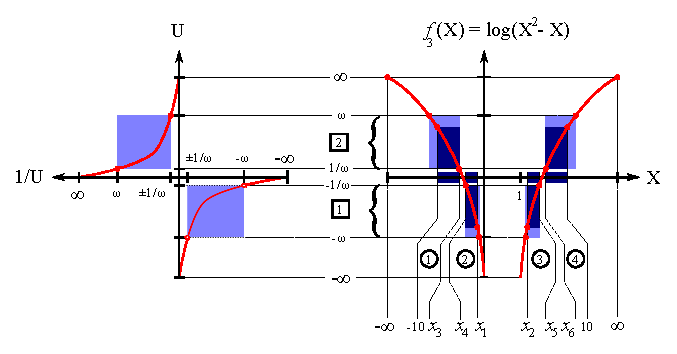
\includegraphics{Images/logX2minusX.eps}
  \caption[Domain of $f_3(X)$]
          {Domain of $f_3(X)$}
  \label{fig:logX2minusX}
\end{figure}

The last step of domain refinement in this example is shown in figure \ref{fig:logX2minusX}. Recall from \ref{fig:ExampleDomains} that the numerical domain of $1/x$ requires a small exclusion interval $C = (-1/\omega, 1/\omega)$. In isolation the primitive reciprocal function is defined on the piecewise domain $\{(-\omega, -1/\omega), (1/\omega, \omega)\}$. In figure \ref{fig:logX2minusX} the domains are \squared{1} and \squared{2} respectively. The pre-images under $f_3$ are then intersected with the domain of refined $f_2$ yielding the refined domain of $f_3$ as
\begin{align*}
\mathcal{D}(f_3) &= \mathcal{D}(f_1(X)) \cap f_3^{-1}(\{(-\omega, -1/\omega), (1/\omega, \omega)\}) \\
                    &= (-10, x_3) \cup (x_4, x_1) \cup (x_2, x_5) \cup (x_6, 10)
\end{align*}
In figure \ref{fig:logX2minusX} the refined domain of $f_3$ is shown as \circled{1}, $\dots$, \circled{4}. Notice that the intervals $(x_3,x_4)$ and $(x_5, x_6)$ were excluded from the the refined domain of $f_2$ and that they are very small and thus likely of negligible probability.


\begin{figure}
  \centering
  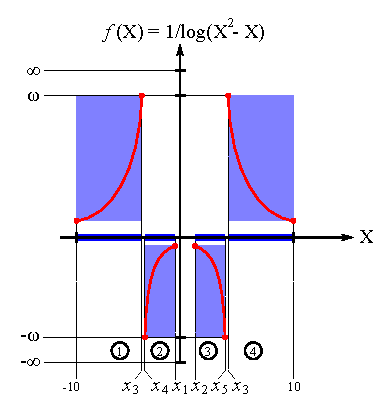
\includegraphics{Images/invlogX2minusX.eps}
  \caption[$Z = f(X)$ with Domain]
          {$Z = f(X)$ with Domain}
  \label{fig:invlogX2minusX}
\end{figure}

Notice that since $f$ does not feed into any other function elements in the example parse tree \ref{fig:invlogX2minusXflow} requires no further refinement. The final function of $f(X)$ is shown in figure \ref{fig:invlogX2minusX} with identified domain \{ \circled{1}, \circled{2}, \circled{3}, \circled{4} \}. 

\subsubsection{Combining Monotonic Functions of Random Variables}

The previous example revealed some important issues in computing functions of random variables. Breaking a function into non-overlapping monotonic fragments begs the question of how to locate interval endpoints. Domain refinement by intersection brought some numerical considerations when values became too small to represent as floating point values. The composition of two bijective functions is a bijective function, but the the same cannot be said for the sum or project of two bijections. The issue of refining a function that is the sum or product of bijections is addressed in this sub-section.

\begin{figure}
  \centering
  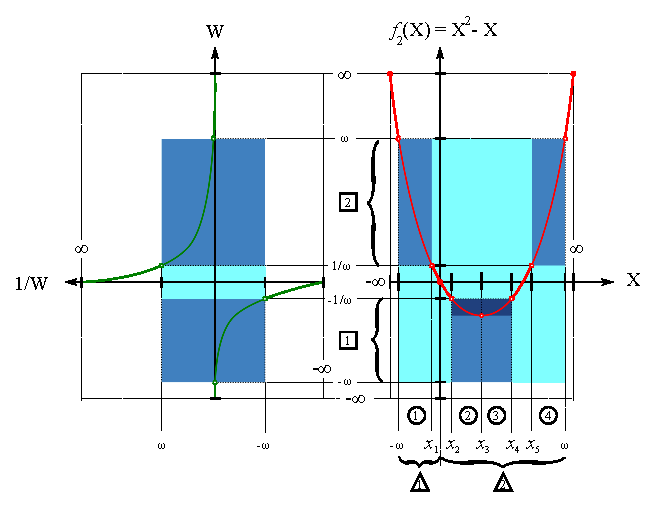
\includegraphics{Images/invX2minusX.eps}
  \caption[Refining $\frac{1}{x^2-x}$]
          {Refining $\frac{1}{x^2-x}$}
  \label{fig:invX2minusX}
\end{figure}

Consider the example,
\begin{align*}
f(x) = \frac{1}{x^2 - x}
\end{align*}
Since $f(x)$ contains $x^2$ the initial domain set is $\{(-\omega,0), (0,\omega)\}$ represented in figure \ref{fig:invX2minusX} by \triangled{1} and \triangled{2} respectively. Recalling the fundamental domain set of $1/x$ from figure \ref{fig:ExampleDomains} as $\{(-\omega, -1/\omega), (1/\omega, \omega)\}$ as \squared{1} and \squared{2} respectively.

Continuing with figure \ref{fig:invX2minusX}, the refined domain element \circled{1} is found by intersecting the pre-image of \squared{2} under $f$ given domain element \triangled{1}. Finding the refined domain element \circled{4} seems just a straightforward; the pre-image under $f$ given domain \triangled{2} intersected with \triangled{2}, but only because $f$ happened to be monotonic in \circled{4}. Notice that $f$ over domain element \triangled{2} is not monotonic. What is required is the intermediate step of refining each original domain element (\triangled{1} and \triangled{2} in this example) so that $f$ is monotonic over each domain element before further refining $f$ against $1/x$.

%%%%%%%%%%%%%%%%%%%%%%%%%%%%%%%%%%%%%%%%%%%%%%%%%%%%%%%%%%%%%%%%%%%%%%%%%%%%%%%%%%%%%%%%%%%
